%DJN: header files
\documentclass{elsart}
\journal{Journal of Mathematical Psychology}
\usepackage{epsfig}
\usepackage{bm}

% ---------- watermark -----------
\usepackage[firstpage]{draftwatermark}
\SetWatermarkAngle{0}
\SetWatermarkFontSize{0.25cm}
\SetWatermarkVerCenter{1.15cm}
\SetWatermarkLightness{0.5}
\SetWatermarkHorCenter{14cm}
\SetWatermarkText{\shortstack[l]{
Myung, J. I., Navarro, D. J. and Pitt, M. A. (2006). Model selection by normalized \\ maximum likelihood. Journal of Mathematical Psychology, 50, 167-179 \\
http://dx.doi.org/10.1016/j.jmp.2005.06.008
}}
\SetWatermarkScale{1}
% -------------------------------

% DJN page margins
\evensidemargin=0cm
\oddsidemargin=0cm
\topmargin=0cm
\textwidth=16cm
\textheight=22cm
\raggedbottom


\newcommand{\efc}{\vspace*{15pt}}

\begin{document}

% DJN: header material
\begin{center} \title{Model selection by normalized maximum likelihood}
\author{{\normalsize Jay I. Myung$^{a,c}$, Danielle J. Navarro$^b$ \and Mark A. Pitt$^a$}}
\address{$^a$Department of Psychology\\Ohio State University \\\vspace*{5mm}$^b$Department of Psychology\\University of Adelaide, Australia
\\\vspace*{5mm}$^c$Corresponding Author\vspace*{-12pt}}
\end{center} \vspace*{20mm}


% DJN: abstract & keywords
\small \hrule {\bf Abstract} \\
\noindent The Minimum Description Length (MDL) principle is an information theoretic approach to
inductive inference that originated in algorithmic coding theory. In this approach, data are
viewed as codes to be compressed by the model. From this perspective, models are compared on their
ability to compress a data set by extracting useful information in the data apart from random
noise. The goal of model selection is to identify the model, from a set of candidate models, that
permits the shortest description length (code) of the data. Since Rissanen originally formalized
the problem using the crude `two-part code' MDL method in the 1970s, many significant strides have
been made, especially in the 1990s, with the culmination of the development of the refined
`universal code' MDL method, dubbed Normalized Maximum Likelihood (NML). It represents an elegant
solution to the model selection problem. The present paper provides a tutorial review on these
latest developments with a special focus on NML. An application example of NML in cognitive
modeling is also provided. \vspace{5pt} \\ {\it Keywords:} Minimum Description Length, Model
Complexity, Inductive Inference, Cognitive Modeling. \normalsize
\begin{frontmatter}
\end{frontmatter}


\clearpage
%%%%%%%%%%%%%%%
%\renewcommand{\baselinestretch}{2}
\small\normalsize

To select among competing models of a psychological process, one must decide which criterion to
use to evaluate the models, and then make the best inference as to which model is preferable. For
models that can be formulated as probability distributions, there exist a range of statistical
model selection methods to assist in this endeavor. The purpose of this paper is to describe the
latest advances in an information theoretic model selection method known as Minimum Description
Length (MDL). We begin by describing the philosophy and assumptions behind MDL. This is followed
by a tutorial on its most recent incarnation Normalized Maximum Likelihood (NML), as well as its
relationship with other selection methods. The paper ends with an application of NML to the
analysis of category learning data.

\section{Statistical Inference as Data Compression: The MDL Approach}

The Minimum Description Length principle (Rissanen 1978, 1989) is a statistical inference method
that originated in information theory (Cover \& Thomas, 1991), in contrast to both
classical-frequentist methods and Bayesian methods which stem from probability theory. In
classical and Bayesian methods we begin with the assumption that there exists a true probability
distribution $f_T(\cdot)$ from which the observed data were sampled, and the goal of statistics is
to develop models that approximate this truth. It follows that the goal of model selection is to
find the model that is closest to the truth. According to the MDL principle, this foundational
assumption is incorrect. Rissanen (2003, p.\ 4) argues that


\begin{quote}
``..such a process can work well if the situation is similar to that in physics, namely, that
there is a `law' which is guessed correctly and which is capable of describing the data
sufficiently well for one to be able to account for the unavoidable deviations [due] to small
random instrument noise \ldots \ In general, however, we do not have enough knowledge of the
machinery that generates the data to convert it into a probability distribution, whose samples
would be statistically similar to the observed data, and we end up in the impossible task of
trying to estimate something that does not exist."
\end{quote}


\noindent According to this view, the question of whether the true distribution $f_T(\cdot)$ even
exists is inherently unanswerable. We are thus ill-advised to base our inferential procedures on
an unjustifiable faith in an unknown truth. In response to this concern, the MDL principle adopts
a very different approach to modeling. It proposes that the basic goal should be to find
regularities in data, and use these regularities to compress the data set so as to unambigiously
``describe it using fewer symbols than the number of symbols needed to describe the data
literally'' (Gr\"{u}nwald 1998, p.\ 6). The more a model permits data compression, the more the
model enables us to discover the regularities underlying the data. Therefore the goal of model
selection is to identify the model that allows the greatest compression of the data. Conceptually,
the intent is not to discover the truth about the world so much as it is to provide the most
concise account of our observations about the world (i.e., data). Although these two viewpoints
sound similar, they lead to somewhat different statistical machinery.\footnote{It is worth noting
that this philosophical position is not inherent to information theory. Other information
theoretic approaches to statistics take a ``subjectivist'' Bayesian view, notably the Minimum
Message Length framework (Wallace \& Boulton, 1968; Wallace \& Dowe 1999a).}

The MDL approach has evolved over the past 30 years from its initial ``two-part" code that was
 limited in applicability, to the more ``modern" and sophisticated form that has made its way
into the psychological literature (Gr\"{u}nwald, 2000; Navarro \& Lee, 2004; Pitt, Myung \& Zhang,
2002). Normalized Maximum Likelihood (NML) is currently the endpoint of this journey, providing a
theoretically elegant solution. Readers interested in more detailed coverage of the material that
follows should consult the tutorial chapter by Gr{\"{u}}nwald (2005), upon which section 2 of this
paper is drawn. A comprehensive summary of recent developments in MDL theory and its application
can be found in Gr{\"{u}}nwald, Myung and Pitt (2005).

\section{Normalized Maximum Likelihood}

We begin with a discussion of the foundational ideas that underlie MDL and NML. We do so to ensure
that this paper is self-contained. An excellent discussion can be found in Gr\"{u}nwald (2000; see
also Li \& Vit\'{a}nyi, 1997), so there is little need to repeat the material in detail.

\subsection{Codes, Codelengths and Probabilities}

Suppose we are presented with a data set $\bm x$ that consists of the sequence of $n$ symbols
 $x_1 \, x_2 \, \ldots\, x_n$. If we are flipping coins, for instance, this could be the binary
sequence
\begin{quote}
\textsc{hhhhhhhththhhthtthhhhhhhhhhh}
\end{quote}
The literal description length of this data set, when written in the
binary \emph{alphabet} (\textsc{h,t}), is $l(\bm x)=n=28$ symbols. However, it may be possible to
devise a different {\it encoding} of the data set that is much shorter. Suppose that we adopt
 a \emph{code} that supposes \textsc{aa=h, ab=t, ba=hhh, bb=hhhh}. This code also uses a
binary alphabet, in this case (\textsc{a,b}), but when we write out the data in code, we obtain
\begin{quote}
\textsc{bbbaabaaabbaabaaababbbbbbb}
\end{quote}
which has a \emph{codelength} of only $l(\bm x)=26$ binary symbols. Notice that an observer who
knows the code can precisely decipher the message. No message written in this code can correspond
to multiple data sets, due to the fact that none of the \emph{codewords} (i.e., \textsc{aa, ab,
ba, bb}) is a prefix of any other, making the code a so-called \emph{prefix code} that guarantees
unique decodability. Moreover, note that the code makes a statement about the kinds of
regularities that we expect to see in the data, namely that there should be more heads than tails.

With this in mind, the key to understanding the MDL principle lies in Shannon's source coding
theorem and in the Kraft inequality. The Kraft inequality states that for any computable
probability distribution $p(\cdot)$ there exists a corresponding prefix code that encodes the data
set $\bm x$  as a sequence of $l(\bm x) =-\! \lceil \log_2 p(\bm x) \rceil$ binary symbols
(``bits''), and vice versa, in such a way that short codewords are assigned to frequent data
symbols and long codewords are assigned to infrequent data symbols. The symbol $\lceil z \rceil$
denotes the smallest integer greater than or equal to $z$. The convention in information theory is
to use a slight idealization that allows non-integer codelengths. It is also commonplace to think
of these idealized codelengths in ``nats'' rather than bits, where a nat refers to an ``alphabet''
that consists of $e$ ``symbols'', so we use the natural logarithm rather than the binary
logarithm. Under these idealizations, the correspondence between codelength functions and
probability distributions is much simpler, since $l(\bm x) =-\! \ln p(\bm x)$. In other words,
there is an exact correspondence between prefix codes and probability distributions. Moreover, for
data sequences generated from the distribution $p(\cdot)$, Shannon's source coding theorem tells
us that this coding scheme is optimal in the sense that it minimizes the expected length of an
encoded data set (Hansen \& Yu, 2001). Using these optimal \emph{Shannon-Fano-Elias} codes,  we
can say that the shortest attainable codelength for the data $\bm x$ is $-\!\ln p(\bm x)$ when
encoded with ``the assistance'' of the probability distribution $p(\cdot)$. To be slightly more
precise, the Kraft inequality allows us to associate the distribution $p(\cdot)$ with the code,
and Shannon's theorem tell us the code would be optimal if the data were actually generated from
this distribution. Taken together, these theorems tell us that when the observed data $\bm x$ are
compressed using this code, the resulting codelength is $-\!\ln p(\bm x)$ and the minimum expected
codelength is achieved for data generated from $p(\cdot)$.

\subsection{Universal Codes and Universal Distributions}

If theoretical models consisted only of a single probability distribution $p(\cdot)$, then these
basic principles of information theory would have provided a complete (and trivial) solution to
the model selection problem. The probability model that best compresses the data is simply the one
that assigns highest probability to those data. That is, choose the model that fits the data best
(in the maximum likelihood sense). However, this is not how real modeling works. Theoretical
models are built with parameters $\bm\theta$ that are allowed to vary from context to context, and
what the model specifies is the conditional distribution $f(\cdot | \bm\theta)$. As a result, the
model is actually a \emph{family} of probability distributions consisting of all the different
distributions that can be produced by varying $\bm\theta$. In this situation, the model selection
problem is substantially more difficult. From an MDL perspective, we would like to compare two
models on their ability to compress the data. However, in order to do so, we need to know how to
optimally encode the data $\bm x$ with the help of an entire family of distributions $M$. The
corresponding codelength is called the \emph{stochastic complexity} (SC) of $\bm x$ with respect
to $M$.

How should we optimally encode the data $\bm x$ with the help of the model family $M$? Notice
that, since the Kraft inequality establishes a correspondence between codes and probability
distributions, this is the same as asking what probability distribution should be used as the most
suitable substitute for the family $M$ when trying to describe the data $\bm x$. An obvious answer
would be to use the code corresponding to $f(\cdot | \hat{\bm \theta})$, where $\hat{\bm \theta}$
is the maximum likelihood estimate for the data $\bm x$, since this distribution assigns shorter
codelength to the data than any of the other distributions in the model family. The problem with
doing so is that the code remains unknown until the data are observed. If person A wishes to
describe $\bm x$ to person B (who has not yet seen the data) using the code corresponding to
$f(\cdot | \hat{\bm \theta})$, then \emph{both} A and B need to know the code, which depends on
$\hat{\bm \theta}$, which in turn depends on the data. Since person B has not yet seen the data,
this is impossible. In other words, since this ``maximum likelihood code'' depends on the data
themselves, it cannot be used to describe those data in an unambiguous (i.e., unique) manner.
Something else is required.

To recap, we wish to identify the single probability distribution that is ``universally"
representative of an entire family of probability distributions in the sense that the desired
distribution mimics the behavior of any member of that family (Barron, Rissanen \& Yu, 1998). The
MDL principle gives guidelines as to how to construct such a distribution. Formally, a {\it
universal distribution} $p_U(\bm x)$ relative to a family of distributions $M$ is defined as a
distribution that allows us to compress every data set $\bm x $ almost as well as its maximum
likelihood code (i.e., $-\ln f(\bm x| \hat{\bm \theta}_{\bm x})) $ in the following sense
(Gr\"{u}nwald, 2005):
\begin{equation}\label{unidist}
-\ln p_U(\bm x) \leq -\ln f(\bm x | \hat{\bm \theta}_{\bm x}) + K_n (M)
\end{equation}
where $K_n(M)$ increases sublinearly in $n$, that is, $\displaystyle\lim_{n \rightarrow \infty}
K_n(M)/n =0$. The {\it Shannon-Fano-Elias} code corresponding to this universal distribution is
called the {\it universal code}. According the equation (\ref{unidist}), the universal code is
nearly as good as the maximum likelihood code, with the difference between the two codes being no
more than $K_n(M)$, yet importantly, the universal code avoids the pitfalls of the `maximum
likelihood code'. Notice that there may exist multiple universal distributions, each with a
different value of $K_n(M)$. We would then be interested in finding the ``optimal" universal
distribution for the model family $M$. The NML solution is presented next.


\subsection{NML as Optimal Universal Distribution}


To understand the NML solution, it is useful to consider how conventional inference methods
conceive the problem. In most statistical frameworks, the problem is addressed by trying to find
the model that is ``closest'' to the true distribution $f_T(\cdot)$ in some well-defined sense.
One natural choice is to measure the discrepancy between the model and the truth using the
Kullback-Liebler divergence (Kullback, 1968),
\begin{equation}\label{kl}
  D(p || f_T)= E_{f_T} \left[ \ln \frac{f_T(\bm x)}{p(\bm x)} \right].
\end{equation}
Information theoretically, the Kullback-Liebler approach is appealing because it measures the
amount of information lost when $p(\cdot)$ is used to approximate $f_T(\cdot)$. This is in the
sense that, when data is generated from $f_T(\cdot)$ and encoded using $p(\cdot)$, an average of
$D(p||f_T)$ additional nats are required beyond what would have been needed had we used the
optimal code specified by $f_T(\cdot)$. Under the information theoretic view, model selection
should aim to find the model that best approximates the truth. This approach (under some very
strong asymptotic assumptions) was used to derive the Akaike Information Criterion (AIC; Akaike,
1973). As such, the approach relies on the assumption that a true distribution really exists. As
mentioned earlier, this assumption is rejected in MDL. It is not simply that the true distribution
is unknown but the assumption of the data generating distribution is ``quite irrelevant to the
task at hand, namely, to learn useful properties from the data" (Rissanen, 1989, p. 17). What this
implies is that the goal of model selection is not to estimate an assumed but `unknown'
distribution, but to find good probability models that help separate useful information in the
data from noise (Rissanen, 1989, p. 84).


In this theoretically conservative approach, how should the problem of inference be redefined to
avoid referring to a true distribution? Firstly, the machinery  available to us in statistics are
probability distributions, so we must work with what we have. Secondly, in order to make ``safe''
inferences about an unknown world, a cautious approach would be to assume a worst-case scenario of
some kind. With this in mind, we return to the original problem, in which we are given a family of
probability distributions to assist us with data coding. Recall that the absolute best performance
that the model family is capable of for any data set $\bm x$ is equal to the minus log maximum
likelihood value, $- \ln f(\bm x |\hat{\bm\theta}_{\bm x})$, but that it is not possible to
specify the corresponding code before observing the data, making it useless for any practical
purpose. We will instead use a universal distribution $p(\bm x)$ to encode the data. The excess
codelength needed to encode the data set $\bm x$ with this universal distribution, $\{ -\ln p(\bm
x) + \ln f(\bm x | \hat{\bm \theta}_{\bm x}) \}$, is called the {\it regret} of $p(\bm x)$
relative to $M$ for the data.

>From a worst-case perspective, the following question is an obvious one to ask: Given a coding
scheme that we can specify in advance which corresponds to the distribution $p(\bm x)$, how
closely does it imitate the impossible scheme implied by $f(\bm x |\hat{\bm\theta}_{\bm x})$ under
the worst conditions (i.e., when the data are generated from a ``worst enemy'' distribution that
makes it hardest for $p(\bm x)$ to approximate $f(\bm x |\hat{\bm\theta}_{\bm x})$)? More
formally, the worst-case expected regret is given by
\begin{equation}\label{regret}
R(p||M)=\max_{q} E_{q}\left[\ln\frac{\displaystyle f(\bm x |\hat{\bm\theta}_{\bm
x})}{\displaystyle p(\bm x)}\right]
\end{equation}
where the ``worst enemy'' distribution $q(\cdot)$ is allowed to be (almost) any probability
distribution.

Comparison of (\ref{kl}) and (\ref{regret}) brings out the differences between the conventional
and MDL approaches to the inference problem. In (\ref{kl}), we assume a true distribution $f_{T}$
that plays two distinct roles: it is both the thing to be approximated (in the numerator), and the
thing that we must assume produces the data (in the expectation). In MDL, we are not allowed to
assume that such a thing exists, and (\ref{regret}) addresses these two roles differently.
Firstly, we cannot approximate a true distribution because we are not allowed to assume such a
thing in the numerator. Instead, we adopt the more modest goal of seeking an optimal coding scheme
based on the various maximum likelihood codes that belong to the model family $M$. In the second
case, we are not allowed to assume that the data are generated by a true distribution, so we adopt
the most cautious approach we can think of, and assume that the data are generated from the
distribution $q$ under which the approximation is poorest.

Without making any reference to the unknown truth, Rissanen (2001) formulated finding the optimal
universal distribution as a minimax problem: Find the coding scheme that minimizes the worst-case
expected regret,
\begin{equation}\label{minimax}
p^* = \displaystyle\arg _{p} \min_{p} \max_{q} E_{q}\left[\ln\frac{\displaystyle f(\bm x
|\hat{\bm\theta}_{\bm x})}{\displaystyle p(\bm x)}\right]
\end{equation}
where $q$ ranges over the set of all probability distributions satisfying $E_{q}\left [ \ln
\frac{q(\bm x)}{f(\bm x |\hat{\bm\theta}_{\bm x})} \right] < \infty$ for all $\bm\theta \in
\bm\Theta$. Neither $p$ or $q$ is required to be a member of the model family, nor is the
solution, $p^*$. The process by which the NML is derived is illustrated in
Figure~\ref{nmlgeometry}. The distribution that satisfies this minimax problem is the
\emph{normalized maximum likelihood} (NML) distribution (Barron, Rissanen \& Yu, 1998; Rissanen,
2001)\footnote{It is interesting to note that the same NML distribution $p^*(\bm x)$ can also be
derived as the solution to another minimax problem defined as $p^* = \displaystyle\arg _{p}
\min_{p} \max_{\bm x } \left(\ln\frac{\displaystyle f(\bm x |\hat{\bm\theta}_{\bm
x})}{\displaystyle p(\bm x)}\right)$ (Shtarkov, 1987). Note that in this minimax formulation, the
worst-case {\it individual data} regret is being minimized, rather than the worst-case {\it
expected} regret as in (\ref{minimax}).},
\begin{equation}\label{nml-mc}
p^*(\bm x) = \frac{f(\bm x |\hat{\bm\theta}_{\bm x})}
{\int  f(\bm{y}|\hat{\bm{\theta}}_{\bm{y}}) \ d\bm{y}}
\end{equation}
where $\hat{\bm{\theta}}_{\bm{y}}$ denotes the maximum likelihood estimate for the data set
$\bm{y}$. Therefore, the probability that this optimal universal distribution $p^*$ assigns to the
data set $\bm x$ is proportional to the maximized likelihood value $f(\bm x
|\hat{\bm\theta}_{\bm{x}})$, and the normalizing constant $\int
f(\bm{y}|\hat{\bm{\theta}}_{\bm{y}}) \ d\bm{y}$  is the sum of maximum likelihoods of all
potential data sets that could be observed in an experiment. It is for this reason that $p^*$ is
called the normalized maximum likelihood distribution. When the data $\bm x$ is defined over a
discrete sample space (e.g., binomial data), the integration symbol $\int$ in (\ref{nml-mc}) is
replaced by the summation symbol $\sum$.\

\begin{figure}[t]
   \begin{center}
   \begin{tabular}{c}
  \includegraphics[height=7.5cm]{nmlgeometry.eps}
   \end{tabular}
   \end{center}
   \caption{A schematic illustration of the minimax problem used to derive NML. Data $\bm x$
are treated as if they were generated from $q$, and the model fit is given by
$f(\cdot|\hat{\bm\theta})$. The optimal distribution $p^*$ minimizes the expected discrepancy from
$p$ to $\hat{\bm\theta}$, under the assumption that the distribution $q$ that generates $\bm x$ is
chosen to maximize this discrepancy.}
 \label{nmlgeometry}
\efc
\end{figure}

The codelength of the normalized maximum likelihood, $-\ln p^*(\bm x)$, is referred to as the
stochastic complexity of the data set $\bm x$ with respect to the model class $M$ and is given by
\begin{equation} \label{nmleq}
\mbox{SC}_1  =  -\ln f(\bm{x}|\hat{\bm{\theta}}_{\bm{x}}) + \ln \int
f(\bm{y}|\hat{\bm{\theta}}_{\bm{y}}) \ d\bm{y} \nonumber.
\end{equation}

In (\ref{nmleq}) the first term of the right hand side is a lack of fit measure and the second
term defines the {\it complexity} of the model class $M$. Thus, in $\mbox{SC}_1$, model complexity
is operationalized as the logarithm of the {\it sum of all best fits} a model class can provide
collectively. A model that fits almost every data pattern very well would be much more complex
than a model that provides a relatively good fit to a small set of data patterns but does poorly
otherwise. This is how the complexity measure captures the model's ability to fit random data sets
(Myung \& Pitt, 1997). Another interpretation of complexity is that it is equal to the minimized
worst-case {\it expected} regret, i.e., the expected regret at $p^*(\bm x)$ (Rissanen, 2001),
\begin{equation} \label{mc}
\ln \int f(\bm{y}|\hat{\bm{\theta}}_{\bm{y}}) \ d\bm{y} = E_{q}\left[\ln\frac{\displaystyle f(\bm
x |\hat{\bm\theta}_{\bm x})}{\displaystyle p^*(\bm x)}\right].
\end{equation}

According to the MDL principle, given a set of competing models, we first use the NML
distributions to compare their ability to compress the data and then select the one model that
minimizes the $\mbox{SC}_1$ criterion.

\begin{figure}[t]
   \begin{center}
   \begin{tabular}{c}
  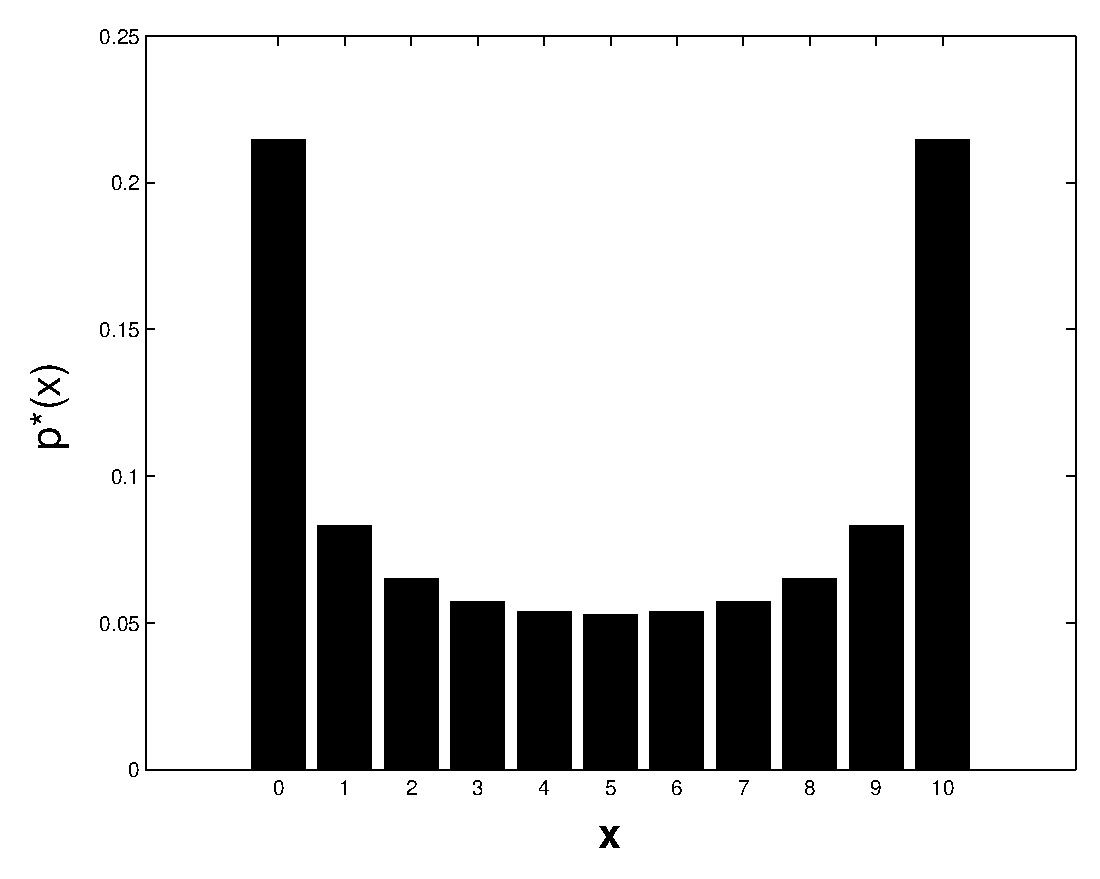
\includegraphics[height=7.5cm]{nml_dist.eps}
   \end{tabular}
   \end{center}
   \caption{The NML distribution for the binomial model class with sample size $n = 10$.}
 \label{nml_dist}
\efc
\end{figure}

To give an example showing how NML distributions are defined, consider the binomial variable $x$
with the probability mass function,

\begin{equation}\label{binomial}
f(x|\theta)=\frac{n!}{x!(n-x)!} \theta^x (1-\theta)^{n-x}
\end{equation}
where $x = 0,1,...,n$ and $0 < \theta < 1$. The maximum likelihood estimate of the parameter
$\theta$ is given by $\hat{\theta} = x/n$. The NML distribution $p^*(x)$ is then defined as
\begin{equation}\label{nml_binomial}
p^*(x) =\frac{ \frac{n!}{x!(n-x)!} {\left( \frac{x}{n} \right)}^x {\left(
\frac{n-x}{n}\right)}^{n-x}} {\sum_{y=0}^{n} \frac{n!}{y!(n-y)!} {\left( \frac{y}{n} \right)}^y
{\left( \frac{n-y}{n}\right)}^{n-y}}.
\end{equation}
For sample size n = 10, the normalizing constant in the denominator of (\ref{nml_binomial}) is
approximately 4.66, the logarithm of which (i.e., $\ln(4.66) = 1.54$) gives the complexity measure
of the model class. Figure~\ref{nml_dist} shows $p^*(x)$ for $n=10$. As can be seen in the figure,
$p^*(x)$ does not resemble any binomial distribution as the NML distribution resides outside of
the model class. Despite this ``misgiving," it is important to note that the NML distribution is
the one that is universally representative of the entire model class in the minimax sense in
(\ref{minimax}).

There are two important caveats concerning the implementation of the stochastic complexity
criterion in (\ref{nmleq}) in practice. First, if the value of the normalizing constant in
(\ref{nml-mc}) is infinite, the NML distribution $p^*$ is then undefined and therefore cannot be
used. This is sometimes known as the {\it infinity problem}, to which there is not yet a fully
general solution, though several remedies have been suggested to `repair' this undesirable
situation (Gr\"{u}nwald, 2005). The problem is currently a topic of active research and discussion
in the field (Rissanen, 2000; Lanterman, 2005; Foster \& Stine, 2005; Wallace \& Dowe, 1999b).

Second, although the complexity measure in (\ref{mc}) is invariant to reparameterizations of the
model, it is not necessarily invariant to different choices of experimental design. To illustrate,
suppose that we have observed 7 heads out of 10 independent Bernouilli trials in a coin tossing
experiment and that we wish to compute stochastic complexity. It turns out that this is not
possible because additional information is needed. That is, different values of the normalizing
constant are obtained depending upon the sampling scheme we assume for the data, whether we had
planned to terminate the experiment after 10 trials regardless of the outcomes (i.e., binomial
sampling) or to continue the experiment until 7 heads are observed (i.e., negative binomial
sampling). Wallace and Dowe (1999b) recently questioned NML-based model selection on the grounds
that this violates the Likelihood Principle (LP; e.g., Berger \& Wolpert, 1988). The LP states
that given a data set $\bm x$, the likelihood function for the data $ f(\bm x| \bm \theta)$
contains all the information about $\bm\theta$. If information about $\bm\theta$ lies outside the
likelihood function such as in how the experiment was carried out or other background information,
it is a violation of this principle (Press, 2003, p. 36). As Edwards, Lindman and Savage (1963, p.
193) argue, ``the rules governing when data collection stops are irrelevant to data
interpretation. It is entirely appropriate to collect data until a point has been proven or
disproven, or until the data collector runs out of time, money, or patience''. However, it is
worth noting that there is some disagreement over the LP in statistics (e.g., Hill, 1987), and
with regard to MDL in particular. In particular, given that MDL focuses on sequentially observed
data transmitted over some channel, it is not obvious whether the stopping rules should be
irrelevant to MDL (Peter Gr\"{u}nwald, personal communication). In short, this remains an issue
for theoreticians to address in the future.


\subsection{Asymptotic Approximations to NML}

Having introduced the NML criterion as an ``optimal'' implementation of the MDL principle,
it is instructive to compare it with a number of
other formulae that have, at different points in time, been referred to as ``the MDL criterion''.
The version of MDL that has been used most frequently in psychology
is the ``Fisher information approximation to the stochastic complexity criterion''. This is the
criterion used by Pitt et al. (2002) and discussed at length
in Gr\"{u}nwald (2000). It has proven to be fairly robust in model selection and is
much more tractable than NML. The expression was derived
by Rissanen (1996) by taking an asymptotic expansion of the complexity term in (\ref{nmleq})
for large sample sizes,
\begin{equation}\label{approx}
\mbox{SC}_2 ~ =~   -\ln f(\bm{x}|\hat{\bm{\theta}}_{\bm{x}}) + \frac{k}{2} \ln \left(
\frac{n}{2\pi} \right) + \ln \int_{\Theta} \sqrt{\det I(\bm{\theta})} \, d\bm{\theta} + o(1)\\
\end{equation}
where $n$ denotes the sample size, $k$ is the number of model parameters, and $I(\bm\theta)$ is
the Fisher information matrix (e.g., Schervish, 1995) of sample size 1 defined as $
I(\bm\theta)_{i,j} = -E_{f(\cdot | \bm\theta)} \left[ \frac{\partial^2 \ln f(\bm x|\bm
\theta)}{\partial\theta_i \partial \theta_j} \right], \ i, j=1,...,k$. The $o(1)$ term collects
all the higher-order terms in the asymptotic expansion, and vanishes as $n \rightarrow \infty$.
The second and third terms together are often referred to as the complexity of the model, albeit
an asymptotic one. Like NML, this complexity measure is reparametrization-invariant and is not
necessarily invariant under changes of experimental design (Wallace \& Dowe, 1999b).


The second and third terms in (\ref{approx}) reveal three dimensions of model complexity: the
number of parameters $k$, the functional form of the model equation as implied by $I(\bm\theta)$,
and the parameter range given by the domain of the integral, $\Theta$. The second term of the
$\mbox{SC}_2$ criterion captures the number of parameters whereas the third complexity term
captures the functional form and the parameter range. Three observations summarize their
contributions to model complexity. First, note that the sample size $n$ appears in the second term
but not in the third. This implies that as the sample size becomes large, the relative
contribution of the third term to that of the second becomes negligible, further reducing
$\mbox{SC}_2$ to another asymptotic expression:
\begin{equation}\label{sc3}
\mbox{SC}_3 ~ =~   -\ln f(\bm{x}|\hat{\bm{\theta}}_{\bm{x}}) + \frac{k}{2} \ln \left(
\frac{n}{2\pi} \right)
\end{equation}
which is one of the early formulations of the MDL principle (Rissanen, 1978 \& 1983). Second,
because the second term of $\mbox{SC}_2$ is a logarithmic function of sample size but a linear function
of the number of parameters, the impact of sample size on model complexity is less dramatic than
that of the number of parameters. Third, the third term in $\mbox{SC}_2$ depends on the parameter ranges
implied by $\Theta$. Since $\sqrt{\det I(\bm{\theta})}$ is a positive scalar,
the larger the parameter range, the greater the complexity of the model.


Returning the discussion to $\mbox{SC}_2$ in (\ref{approx}), the comparative tractability and ease
of interpretability of this criterion make it a tempting alternative to the NML. However, there
are some important caveats that are often neglected in applied contexts, relating to regularity
conditions. As Rissanen (1996) remarks, in order to apply this expression, the most important
things to verify are that:
\begin{itemize}
\item The maximum likelihood estimate must lie ``sufficiently'' in the interior of the model. That is,
for some $\epsilon > 0$ and for all large $n$, the best fitting parameter value $\hat{\bm
\theta}_{\bm x}$ must be further than $\epsilon$ from the edge of the parameter space;
\item All elements of the Fisher information matrix $I(\bm{\theta})$ must be continuous in $\Theta$;
\item The Fisher information integral term $\int_{\Theta} \sqrt{\det I(\bm{\theta})} \, d\bm{\theta}$ must
be finite.
\end{itemize}
If these conditions are violated, then the stochastic complexity $\mbox{SC}_2$ is not well-defined and
may exhibit anomalous behavior (see Navarro, 2004 for an example). Rissanen (1996; see also
Lanterman, 2001, 2005) discusses several `repair' methods for handling such situations. For
example, a small neighborhood around singular points of $I(\bm{\theta}) =\infty$ may be excluded
from the computation, or the range of parameters may be restricted in order to make the Fisher
information integral finite.


\subsection{Relationships to Bayesian Formulae}
Interestingly, one can also interpret the two asymptotic approximations, $\mbox{SC}_2$ and
$\mbox{SC}_3$, from a Bayesian viewpoint. In Bayesian statistics (Gelman, Carlin, Stern \& Rubin,
2004), the goal of model selection is to choose, among a set of candidate models, the one with the
largest value of the marginal likelihood defined as
\begin{equation}\label{marginal}
p_{_{Bayes}}(\bm x)~=~\int_{\bm\Theta} f(\bm x|\bm \theta) \pi(\bm \theta) d\bm \theta
\end{equation}
where $\pi(\bm\theta)$ is a prior density for the parameter $\bm\theta$. The term {\it Bayes
factor} (Kass \& Raftery, 1995), which is often mentioned in Bayesian model selection, is referred
to as the ratio of the marginal likelihood of one model to the marginal likelihood of a second
model. An asymptotic expansion of the minus log marginal likelihood using the `non-informative'
Jeffreys' prior $\pi_J (\bm\theta) = \sqrt{I(\bm\theta)} / \int_{\bm\Theta} \sqrt{I(\bm\theta)}
d\bm\theta$ yields (Balasubramanian, 1997, 2005)
\begin{equation}\label{margasym}
- \ln p_{_{Bayes}}(\bm x) ~ =~   -\ln f(\bm{x}|\hat{\bm{\theta}}_{\bm{x}}) + \frac{k}{2} \ln
\left(\frac{n}{2\pi} \right) + \ln \int_{\Theta} \sqrt{\det I(\bm{\theta})} \, d\bm{\theta} + o(1)\\
\end{equation}
which is exactly the same as $SC_2$ in (\ref{approx}). Hence, for large $n$, Bayesian model
selection with Jeffreys prior and NML become virtually indistinguishable. Obviously, this
asymptotic ``equivalence" would not hold if a different form of prior is used or if the sample
size is not large.


By neglecting the sample-size independent terms in the right-hand side of (\ref{margasym}) and
then multiplying the result by factor 2, we get another asymptotic expression
\begin{equation}\label{bic}
- 2\ln p_{_{Bayes}}(\bm x) ~ \approx~   -2\ln f(\bm{x}|\hat{\bm{\theta}}_{\bm{x}}) + k \ln n. \\
\end{equation}
This is known as the Bayesian Information Criterion (BIC; Schwarz, 1978) and is essentially the
same as $SC_3$ in (\ref{sc3}).


One closing word of caution. Despite the similarities in asymptotic expressions, Bayesian
inference and MDL are different in their formulations: the marginal likelihood in Bayesian
statistics is not the same as the normalized maximum likelihood in MDL. Therefore they will
generally give different results. For further discussions on the relationships between Bayesian
inference and MDL, the reader is directed to Gr\"{u}nwald (2005) and Vit\'{a}nyi \& Li (2000).



\subsection{Predictive Inference and the MDL Principle}


Predictive inference and data compression are often interchangeable terms in model selection.
Quoting Vit\'{a}nyi and Li (2000, p.~448),``compression of descriptions almost always gives optimal
predictions." That said, stochastic complexity and methods of predictive inference have different
origins. In the predictive approach to model selection, the ultimate goal is the minimization of
prediction errors, and selection criteria differ from one another in how prediction errors are
conceptualized and measured (Geisser \& Eddy, 1979; Geisser, 1993; Linhart \& Zucchini, 1986;
Zucchini, 2000). Many of the non-MDL model selection criteria, such as AIC, cross-validation
(Stone, 1974) and bootstrap model selection (Efron, 1983) were derived as generalizability
criteria in which one is concerned with identifying a model family that yields the best future
predictions. Stochastic complexity, on the other hand, is motivated from a coding-theoretic view
of model selection in which the goal is to identify a model family that permits the tightest
compression of a data set by effectively filtering out random noise and attending to all of the
`useful' information in the data.

It turns out that there are close ties between these seemingly disparate approaches to model
selection, predictive inference in one hand and data compression on the other.The predictive
interpretation of the stochastic complexity has its root in the {\it prequential
analysis} pioneered by Dawid (1984, 1992). To motivate this analysis, let us assume that data $\bm
x^t = (x_1,..., x_t)$ are observed sequentially $\{ 1,...,t \}$ and that we are
interested in predicting the next observation $\bm x^{t+1}$ on the basis of the data observed so
far, that is, $\bm x^t$. Let $\hat {\bm \theta} (\bm x^t)$ denote the maximum likelihood estimate
of a model class $M$ for the data vector $\bm x^t$. Suppose that we use this estimate to predict
the next observation $\bm x^{t+1}$ and further, that we evaluate performance of the maximum
likelihood estimate by the logarithmic loss function, $-\ln f(\bm x^{t+1}|\bm x^t, \hat {\bm
\theta} (\bm x^t))$. The accumulated prediction error (APE) over a series of observations $ t = 1,...,n$
is then given by
\begin{equation}\label{preq}
\mbox{APE}(\bm x^n) = -\sum_{t=0}^{n-1} \ln f(\bm x^{t+1}|\bm x^t, \hat {\bm \theta} (\bm x^t))
\end{equation}
(See Wagenmakers, Gr\"{u}nwald and Steyvers (2005) for a tutorial on APE, along with application
examples in time-series analysis.) It has been shown that the expression in (\ref{preq})
essentially reduces to $\mbox{SC}_3$ in (\ref{sc3}) as $n \rightarrow \infty$ under regularity
conditions (Rissanen, 1986, 1987; Dawid, 1992; Gr\"{u}nwald \& de Rooij, 2005).\footnote{The
primary regularity condition required for the equivalence proof is that the maximum likelihood
estimate $\hat {\bm \theta} (\bm x^t)$ satisfies the central limit theorem such that the tail
probabilities are uniformly summable in the following sense: $P \left(\sqrt{n}
\parallel \hat {\bm \theta} (\bm x^t) -\bm \theta \parallel \geq n \right) \leq \delta(n)$ for all
$\bm \theta$ and $\sum_n \delta(n) < \infty$ where $\parallel \bm \theta \parallel$ denotes a norm
measure (Rissanen, 1986, Theorem 1). Recently, Gr\"{u}nwald and de Rooij (2005) identified another
important condition for the asymptotic approximation, i.e., that the model is correctly specified.
According to their investigation, under model mis-specification, one can get quite different
asymptotic results.} An implication of this observation is that the model that permits the
greatest compression of the data is also the one that minimizes the accumulated prediction error,
thereby providing justification for stochastic complexity as a predictive inference method, at
least asymptotically.


\section{Using NML in Cognitive Modeling}


To provide an application example of NML in cognitive modeling, we consider the seminal experiment
in human category learning conducted by Shepard, Hovland and Jenkins (1961). In this
study, human performance was examined on a category learning task involving eight stimuli divided
evenly between two categories. The stimuli were generated by varying exhaustively three binary
dimensions such as (black, white), (small, large) and (square, triangle). Shepard et al.\ observed
that, if these dimensions are regarded as interchangeable, there are only six possible category
structures across the stimulus set. This means, for example, that the category structure that
divided all black stimuli into one category, and all white stimuli into the other would be
regarded as equivalent to the category structure that divided squares from triangles. These
category structures are shown in Figure \ref{shj-stimuli}.


\begin{figure}[t]\begin{center}\begin{tabular}{c}
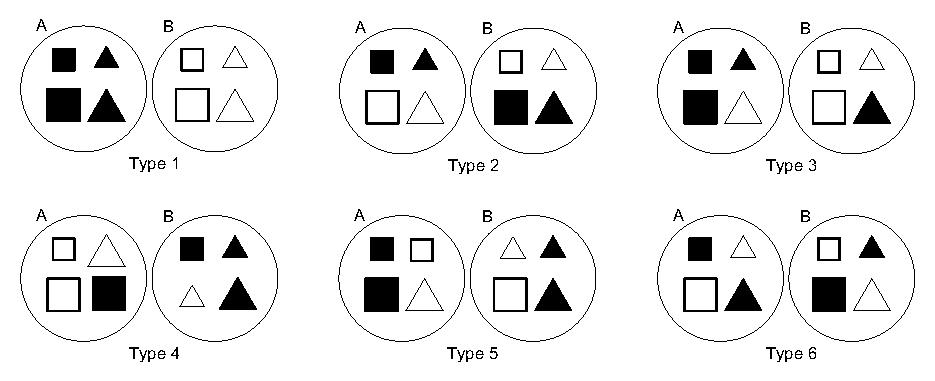
\epsfig{file=shj-stimuli2.eps, width=13.5cm}
\end{tabular}\end{center}
\caption[example]{\label{shj-stimuli} The six category structures that comprise the Shepard,
Hovland and Jenkins task.} \efc
\end{figure}


Empirically, Shepard et al.\ found robust differences in the way in which each of the six
fundamental category structures was learned. In particular, by measuring the mean number of errors
made by subjects in learning each type, they found that Type 1 was learned more easily than Type
2, which in turn was learned more easily than Types 3, 4 and 5 (which all had similar error
rates), and that Type 6 was the most difficult to learn. This result was recently replicated in
Nosofsky, Gluck, Palmeri, McKinley and Glauthier's (1994) work. Figure~\ref{shj} shows the
category learning curves from this experiment. The consensus in the literature is that the ordinal
constraint $1<2<(3, 4, 5)<6$ represents an important and robust property of human category
learning. As a result, the ability to reproduce this ordinal constraint is required in order for a
model to be taken seriously by researchers.


In order to claim that a category learning model reproduces this ordinal constraint, we need to be
able to find a set of equivalence relations among learning curves (whether these be empirical or
predicted curves). This is essentially a partitioning problem. Traditionally, the extraction of
the partition from data has been done subjectively, by the visual inspection of the curves in
Figure~\ref{shj}. However, this is a somewhat unappealing way to justify the partition,
particularly given its importance to category learning. It would be preferable to extract the
partition using principled statistical methods. This becomes especially important for data sets
that do not lend themselves to simple visual displays.


\begin{figure}[t]\begin{center}\begin{tabular}{c}
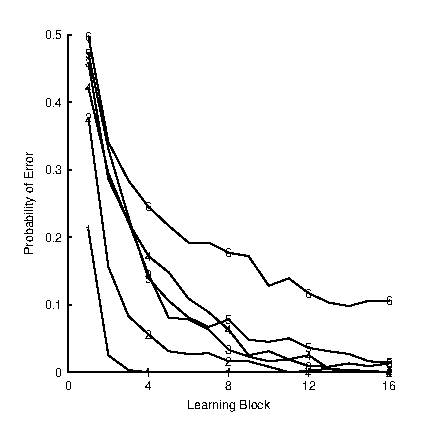
\includegraphics[height=8cm]{shj.eps}
\end{tabular}\end{center}
 \caption[example]
{\label{shj} Empirical learning curves for the Shepard, Hovland and Jenkins task (from Nosofsky et
al., 1994).}
\efc
\end{figure}


To address this, we applied a clustering procedure in which the optimal partition is the one that
maximizes the NML. In order to do so, we treat a clustering solution as a statistical model for
the data, in this case a multivariate binomial model. The problem of choosing the partition now
reduces to the problem of choosing among a set of statistical models, a problem for which NML is
known to be an appropriate solution. Under a model-based clustering procedure, the data are
treated as the outcome of some random process. A clustering solution is thus treated as a
\emph{model} for the data, and the adequacy of that solution can be assessed using statistical
model selection tools. In this section we outline a clustering model for discrete data that is
appropriate to the applied problem of partitioning learning curves.


\subsection{A Partitioning Model}


Suppose that we have a discrete data set made up of $T$ samples, each of which is an $M$-variate
discrete probability over $H$ response options. For instance, we might have $T$ participants who
solve $M$ different kinds of problems, and each problem has $H$ possible answers. Note that since
each class of problem may have a different number of potential responses, $H$ should technically
be denoted $H_m$. However, this subscript will be dropped, since it will be clear from context. A
particular partitioning of these $T$ samples might be expressed in the following way. If we assume
that there are $K$ clusters, we might let $D_k$ indicate how many of the original samples fall
into the $k$th cluster. So $D_k$ represents the size of the cluster, and thus $\sum_k D_k = T$. As
before, we will generally drop the subscript $k$ when discussing $D$.


We represent the data $\bm{x}$ in terms of the statistics $x_{11}^{11} \ldots x^{KM}_{DH}$, where
$x^{km}_{dh}$ counts the number of observations that fall into the $h$th response category on the
$m$th dimension for the $d$th sample that belongs to the $k$th cluster. In the example given
earlier, $x^{km}_{dh}$ would denote the number of times that participant $d$ of cluster $k$ gave
the response $h$ to a problem of type $m$. It will be convenient to define $y^{km}_h$ and $w^{km}$
as $y^{km}_h = \sum_{d=1}^D x^{km}_{dh},\ w^{km} = \sum_{h=1}^H y^{km}_h$.
In the example discussed, $y^{km}_h$ is the number of times that someone in the
$k$th cluster gave the answer $h$ to a problem in $m$, while $w_{km}$ is the total number of times
that a problem of type $m$ was presented to group $k$. A partitioning model for $\bm{x}$ consists
of the set of $K$ clusters $\bm{C}=(\bm{c}_1 \ldots \bm{c}_K)$. In this expression, $\bm{c}_k$
denotes the set of (indices of) samples that belong to the $k$th cluster. The model parameters
$\bm{\theta} = (\theta^{11}_1, \ldots \theta^{MK}_H)$ correspond to the probabilities with which
each of the responses are chosen. Accordingly, ${\theta}^{mk}_h$ gives the probability with which
response $h$ is predicted to occur in trials belonging to cluster $k$ and dimension $m$. Thus the
likelihood $p(\bm{x}|\bm{\theta})$ is,
\begin{displaymath}
p(\bm{x} | \bm{\theta})
= \prod_{m=1}^M \prod_{k=1}^K \prod_{d=1}^D \prod_{h=1}^H (\theta^{km}_{h})^{x^{km}_{dh}}
= \prod_{m=1}^M \prod_{k=1}^K \prod_{h=1}^H (\theta^{km}_h)_{.}^{y^{km}_h}
\end{displaymath}
%\begin{eqnarray*}
%p(\bm{X} \condon \bm{\theta})
%&=& \prod_{m=1}^M \prod_{k=1}^K \prod_{d=1}^D \prod_{h=1}^H (\theta^{km}_{h})^{x^{km}_{dh}} \\
%&=& \prod_{m=1}^M \prod_{k=1}^K \prod_{h=1}^H (\theta^{km}_h)^{y^{km}_h}.
%\end{eqnarray*}
\noindent Note the $y^{km}_h$ values are sufficient statistics for the data, assuming that the
model is $\bm{C}$.


Besides the stipulation that observations come partially pre-clustered in samples, the main
difference between this model class and that used by Kontkanen et al.~(2005) is they employ a
finite mixture model, in which the assignment of items to clusters is assumed to be the result of
a latent probabilistic process. Motivated by the learning curves problem, we assume that a cluster
is a \emph{fixed} grouping of samples. Since the category structures that elicit the samples are
derived from the fixed representational structure of the stimuli (Shepard et al., 1961), it makes
little sense in this context to propose a model class in which object assignments are assumed to
result from a probabilistic process. We now discuss how the NML computations are performed, and
show that the results obtained by Kontkanen et al. (2005) apply to the current model. Since the
current partitioning model is only a very minor variant on the approach adopted by Kontkanen et
al. (2005), we provide only the most basic coverage, and refer interested readers to the original
paper for a more detailed discussion.


For our clustering model, the MLE is given by $\hat{\theta}^{km}_h = \frac{y^{km}_h}{w^{km}}$.
Substituting the MLE values into the likelihood function gives the maximized likelihood,
\begin{eqnarray*}
p(\bm{x} | \hat{\bm{\theta}}_{\bm x}) &=& \prod_{m=1}^M \prod_{k=1}^K \left( \frac{ \prod_{h=1}^H
(y^{km}_h)^{y^{km}_h}}{(w^{km})^{w^{km}}} \right).
\end{eqnarray*}
This will enable us to efficiently calculate the NML value for any data set $\bm{x}$ when
described using a clustering model $\bm{C}$ as
\begin{displaymath}
p_{\mbox{\tiny NML}}(\bm{x}|\bm{C}) = \frac{p(\bm{x}|\hat{\bm{\theta}}_{\bm x})}{\sum_{\bm{y}}
p(\bm{y}| \hat{\bm{\theta}}_{\bm y})}.
\end{displaymath}
In the denominator term, the sum is taken over all possible data sets and represents the
normalizing constant, denoted $\mathcal{R}_{\bm{C}} = \sum_{\bm{y}}
p(\bm{y}|\hat{\bm{\theta}}_{\bm{y}})$.


\noindent The normalizing constant for a clustering model $\bm{C}$ is given by,
\begin{eqnarray*}
R_{\bm{C}} &=& \sum_{y^{11}_{1}+ \ldots +y^{11}_{H} = w^{11}}  \ldots \sum_{y^{KM}_{H}+
\ldots +y^{KM}_{H} = w^{KM}}  \left[ \prod_{m=1}^M \prod_{k=1}^K \frac{w^{km}!}{\prod_{h=1}^H y^{km}_{h}!}
\right]  \left[ \prod_{m=1}^M \prod_{k=1}^K  \frac{ \prod_{h=1}^H (y^{km}_{h})^{y^{km}_{h}}}{(w^{km})^
{w^{km}}} \right],
\end{eqnarray*}
\noindent where the first square-bracketed term counts the number of data sets that have the
sufficient statistics $y^{11}_{1} \ldots y^{KM}_{H}$, and the second square-bracketed term gives
the maximized likelihood to any such data set. After rearranging:
\begin{eqnarray*} R_\mathbf{C} &=& \sum_{y^{11}_{1}+ \ldots +y^{11}_{H} = w^{11}}  \ldots \sum_{y^{KM}_{1}+
\ldots +y^{KM}_{H} = w^{KM}}  \left[ \prod_{m=1}^M \prod_{k=1}^K
\frac{w^{km}!}{(w^{km})^{w^{km}}} \prod_{h=1}^H  \frac{(y^{km}_h)^{y^{km}_{h}}}{y^{km}_{h}!}
\right]. \end{eqnarray*} \noindent Notice that any particular inner term depends on only a single
value of $m$ and $k$. Thus terms where $m=1$ and $k=1$ may be moved forward. Now, notice that all
of the nested terms do not depend on the values of $y^{11}_{1} \ldots y^{11}_{H}$, so they can be
removed as a factor. Repeating this for all $m$ and $k$ allows the normalizing constant to be
factorized, yielding
\begin{eqnarray*}
R_\mathbf{C} &=&\prod_{m=1}^M \prod_{k=1}^K \left[ \sum_{y^{mk}_{1}+ \ldots +y^{mk}_{H} = w^{mk}}
\frac{w^{km}!}{(w^{km})^{w^{km}}} \prod_{h=1}^H  \frac{(y^{km}_h)^{y^{km}_{h}}}{y^{km}_{h}!}
\right]. \end{eqnarray*} \noindent Since individual clusters and dimensions are assumed to be
independent, it is not surprising to see the normalizing constant factorize. The inner term
corresponds to the normalizing constant $R(H,w)$ for a one-dimensional multinomial with $H$
options and a sample size of $w$. That is, $R_\mathbf{C} = \prod_m \prod_k R(H_m,w^{mk})$. The
problem of calculating multinomial normalizing constant is addressed by Kontkanen et al.~(2005),
 so it suffices simply to restate their result:
\begin{eqnarray*}
R(H,w) &=& \sum_{r_1 + r_2 = w} \left( \frac{w!}{r_1!r_2!} \right) \left( \frac{r_1^{\, r_1} r_2^{\, r_2}}
{w^w}  \right)   R(J_1,r_1) \, R(J_2,r_2),
\end{eqnarray*}
\noindent where $J_1$ and $J_2$ are any two integers between 1 and $H-1$ such that $J_1 + J_2 =
H$. They use this result to calculate $R(H,w)$ efficiently using a recursive algorithm. In
essence, we start by calculating all the binomial normalizing constants $R(2,1), \ldots R(2,w)$.
This is reasonably fast since there are comparatively few ways of dividing a sample across two
responses. Once these are known, they can be used to construct the normalizing constants for
larger multinomials. For example, if we needed $H=14$, we would set $J_1=2$ and $J_2=2$ to arrive
at the normalizing constants for $H=4$. We could then set $J_1=4$, and $J_2=4$ to get $H=8$. Then
$J_1=8$ and $J_2=4$ gives $H=12$, and finally $J_1=12$ and $J_2=2$ would give the normalizing
constant for $H=14$. Obviously, at each step we need to calculate the sum over $r_1$ and $r_2$,
but this can be done quickly by constructing tables of normalizing constant values. Once we have
the normalizing constants for the various multinomials, we merely need to take the appropriate
product to get the normalizing constant for the clustering model.

\renewcommand{\baselinestretch}{1}
\small\normalsize
\begin{table}[t]
\begin{center}
\caption{Six clustering solutions to the Shepard et al.\ (1961) problem.} \label{shjclus}
\begin{tabular}{cccc}\\
\hline
Partition & Lack of Fit & Complexity  & $SC_1$ \\
& $\left( -\ln f(\bm{x}|\hat{\bm{\theta}}_{\bm x}) \right)$ &
 $\left( \ln \int f(\bm{y}|\hat{\bm{\theta}}_{\bm{y}}) d\bm{y} \right)$  & \\
\hline
(1, 2, 3, 4, 5, 6) & 16,337 & 70  & 16,408 \\
(1, 2, 3, 4, 5)(6) & 15,399 & 126 & 15,525 \\
(1, 2)(3, 4, 5)(6) & 14,772 & 185 & 14,957 \\
(1)(2)(3, 4, 5)(6) & 14,597 & 237 & 14,834 \\
(1)(2)(3, 5)(4)(6) & 14,553 & 291 & 14,844 \\
(1)(2)(3)(4)(5)(6) & 14,518 & 343 & 14,861 \\
\hline
\end{tabular}
\efc
\end{center}
\end{table}



\subsection{Partitioning Learning Curves}


Nosofsky et al.'s (1994) data have the following properties: each data point is a pooled set of
$n=40\times 16 = 640$ binary observations, assumed to be the outcome of independent Bernoulli
trials. Each of the six curves consists of 16 data points, corresponding to 16 different
measurement intervals. Table~\ref{shjclus} shows the results of the SC calculations for a few
selected clustering solutions. For each solution, the lack of fit measure and the complexity
measure of SC are shown in the second- and the third-columns, respectively, and the overall SC
value is shown in the last column. Note that as we increase the number of clusters, the value of
the lack of fit goes down (i.e., better fit) while the corresponding value of the complexity term
goes up, nicely illustrating the trade-off between these two opposing forces. The SC results in
Table~\ref{shjclus} agree with the intuition that the correct clustering should be
(1)(2)(3,4,5)(6), with the five-cluster solution (1)(2)(3,5)(4)(6) as the closest competitor.
Inspection of Figure~\ref{shj} agrees with this, since the curve for Type 4 is a little different
from those for Types 3 and 5, but the discrepancy is not of the same order as those corresponding
to Types 1, 2 and 6. In short, the SC-based clustering procedure is ``correctly" partitioning this
data set.


%\subsection{Human Category Learning and Stimulus Coding}


%Theoretical work on human classification stresses the importance of  data compression. It is
%assumed that humans make classification decisions not only to make predictions about the world,
%but to efficiently code the information in the environment. In the last section we demonstrated
%that there is strong empirical evidence that the Shepard curves should indeed be partitioned as
%(1)(2)(3,4,5)(6). In \cite{feldman00} the corresponding partial order 1$<$2$<$(3,4,5)$<$6 was
%shown to reflect the amount of information carried by each category structure, so it appears that
%the rate at which humans acquire a category is well-predicted by the informational content of the
%category. Given the obvious theoretical importance of this regularity, an interesting test of the
%validity of category learning models is the extent to which they preserve this regularity across
%their parameter spaces. If different parameterizations of a model are intended to correspond to
%different kinds of plausible human performance, then they should not violate this ordering too
%severely.
%
%We tested this proposition with regard to the classic ALCOVE model \cite{kruschke92}, which learns
%by backpropagating the error made by an adaptive kernel density estimator. In order to search
%ALCOVE's parameter space, we used the Markov chain Monte Carlo algorithm proposed in \cite{kim04}
%to find the different partial orders predicted by the model (see \cite{pitt05} for details). In
%total, there are only eleven stable orderings that occupy a substantial proportion of the
%parameter space,  one of which is the empirically observed order. From this, it is clear that
%Types 3 and 4 are always (11 of 11) predicted to be learned at about the same rate, and Type 5 is
%usually (9 of 11) also about the same. Type 6, on the other hand, is mostly learned slower than 3,
%4 and 5 (8 of 11). Types 1 and 2 are usually (8 of 11) slower than 3--5. So, not only is the
%empirically-observed ordering  among the most common predictions, but the other high-frequency
%predictions generally preserve most of the pairwise relations implied by the empirical data. The
%exception to this claim regards the relationship between Types 1 and 2. In this regard, the model
%predictions are ambiguous. It might be that $1<2$ (4 of 11), or $1=2$ (4 of 11), or even $2<1$ (3
%of 11). In this case, ALCOVE does not make a strong prediction about the relationship between
%informational content and category learning.


\subsection{Revisiting Model Complexity}


Accounting for model complexity is an important topic in statistics (e.g., Hastie et  al., 2001;
Myung, 2000) with clustering models receiving particular attention in applied work (Lee, 2001; Lee
\& Navarro, 2005). Unfortunately, many approaches to model selection rely on asymptotic criteria
such as AIC (Akaike, 1973) or BIC (Schwarz, 1978), or else do not provide an explicit measure of
model complexity (e.g., Bayes factors; see Kass \& Raftery, 1995).  As a result, a great deal of
the discussion of complexity and model selection has relied on asymptotic measures (e.g., Pitt et
al., 2002) that can be misleading in finite samples or when regularity conditions are violated
(Lanterman, 2001; Navarro, 2004). In contrast the NML criterion is exact, and optimal (in the
minimax coding sense discussed earlier) for data of any sample size. Moreover, it supplies a
natural complexity measure (i.e., $\ln R$). Taken together, these two properties allow us to
measure complexity properly and discuss it accurately.


\begin{figure}\begin{center}
\begin{tabular}{cc}
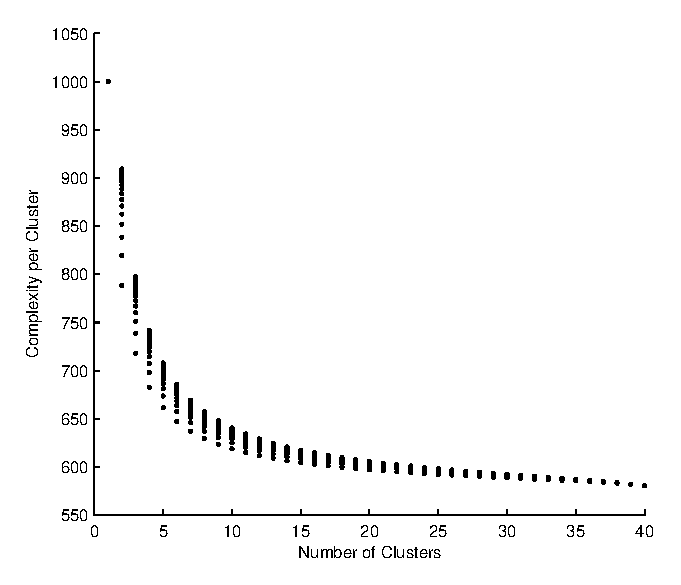
\epsfig{file=complexity.eps,width=7cm} &
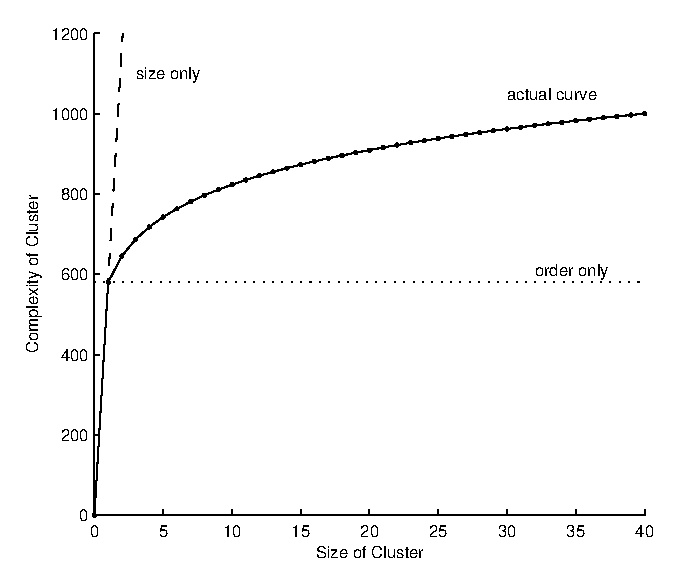
\epsfig{file=complexity3.eps,width=7cm}\\
(a) & (b)
\end{tabular}
\caption{Understanding model complexity. In panel a, we see that model complexity per cluster
$(1/K)\ln R$ is not constant, either as the number of clusters changes or within a fixed model
order. In panel b, we note that complexity associated with a particular cluster increases with
size (solid line). The dotted line (``order only'') shows the predicted curve if only the number
of clusters contributed to complexity. The dashed line (``size only'') shows the predicted curve
if complexity related only to the size of the clusters.} \label{complexity} \efc
\end{center}\end{figure}


It has often been argued (e.g., Lee, 2001; Lee \& Navarro, 2005; Pitt et al. 2002) that model
complexity is not the same as model order. However, these assertion have usually relied on
asymptotic criteria: In a clustering context, Lee (2001) used a Laplace approximation to the Bayes
factor (see Kass \& Raftery, 1995), while Lee and Navarro (2005) used the Fisher information
approximation to MDL. Using the recursive algorithm to calculate exact NML complexities for
clustering models, it is worth briefly revisiting the question. Figure~\ref{complexity}a plots NML
complexity per cluster $(1/K)\ln{R}_{\bm{C}}$ against the number of clusters $K$ for every
possible partition of $T=40$ samples, with $H=20$ response options, $N=100$ observations per cell,
and $M=16$ dimensions. If complexity is well-captured by the number of parameters,
$(1/K)\ln{R}_{\bm{C}}$ should be constant. Figure~\ref{complexity} shows that complexity per
cluster is not constant as $K$ increases, nor is it constant across models with the same number of
clusters. As suggested by Lee (2001), some partitions are indeed more complex than others even
when the total number of clusters remains constant. The reason for this pattern becomes clearer
when we consider the relationship between the size of a cluster (i.e., the number of samples
assigned to it) and its complexity. Figure~\ref{complexity}b plots this relationship for clusters
of the same data sets referred to in Figure~\ref{complexity}a (i.e., $T=40$, $H=20$, $N=100$ and
$M=15$). The dotted line is the predicted curve if complexity were a constant function of model
order, and the dashed line shows the prediction if complexity were a constant function of cluster
size (in fact, if the dashed line were accurate, then each observation would contribute equally to
complexity irrespective of how they were partitioned, and all clustering solutions would be of
equal complexity). However, the figure shows that complexity is a concave increasing function of
cluster size. If model complexity were equivalent to model order, this function would be constant,
ensuring that all clusters contribute the same amount of complexity irrespective of size. Since
the function is increasing, two clusters of size 1 are simpler than two clusters of size 2.
Moreover, since the function is concave, complexity is subadditive. As a result, complexity is
always decreased by transferring an observation from a small cluster to a large one, implying that
the least complex solution is one in which all clusters except one are of size 1, while the
remaining cluster is of size $T-K+1$. This agrees with results based on Laplacian approximations
(Lee, 2001).


\section{Conclusion}


In any scientific context we are presented with limited information that is consistent with an
infinite number of explanations, but are required to infer the ``best'' account in spite of our
limitations, and make ``safe'' inferences about future events. There may indeed be ``more things
in heaven and Earth \ldots than are dreamt of in [our] philosophy'', as Hamlet would have it, but
this does not alleviate the fundamental need to understand the environment and behave
appropriately within it. From a model selection standpoint, the MDL perspective has the appeal
that it avoids making the assumption that the truth ever lies within the set of models that we
might consider. In fact, it does not rely on the notion that there even exists any ``true''
distribution that generates the data. Instead, it relies solely on the efficient coding of
observations. By capturing the regular structure in the data that are observed, we seek to
generalize better to future data without ever invoking the notion of ``the truth''.


%%%%%%%%%%%%%%%%%%%%%%%%%%%%%%%%%%%%%%%%%%%%%%
%%%%%%%%%%%%%%%


\section*{Author Notes}


Correspondence address: Jay Myung, Department of Psychology, 238 Townshend Hall, 1885 Neil Avenue
Mall, Columbus, Ohio 43210-1222, USA. E-mail: myung.1@osu.edu; Voice: 614-292-1862; Fax:
614-688-3984. JIM and MAP were supported by NIH grant R01 MH57472. DJN was supported by Australian
Research Council grant DP-0451793. Portions of this research were presented at the 2005 Electronic
Imaging Conference held in San Jose, CA and were subsequently published in the Proceedings. Other
parts of the work have been submitted to the 2005 IEEE Information Theory Symposium held in
Adelaide, Australia. The authors wish to thank three anonymous reviewers for many helpful
suggestions on an earlier version of this manuscript.


%%%%%%%%%%%%%%%%%%%%%%%%%%%%%%%%%%%%%%%%%%%%%%
%%%%%%%%%%%%%%%
%%%%% References %%%%%


%\bibliography{report}   %>>>> bibliography data in report.bib
%\bibliographystyle{spiebib}   %>>>> makes bibtex use spiebib.bst

\section*{References}
\vspace*{2pt}
%\footnotesize
\begin{list}{}{\setlength{\leftmargin}{12pt}\setlength{\itemindent}{-12pt}\setlength{\parsep}{0pt}}
\item Akaike, H. (1973). Information theory and an extension of the maximum likelihood principle.
In B. N. Petrov \& F. Csaki (eds), {\it Second International Symposium on Information Theory, pp.
267--281}. Budapest: Akademiai Kiado.
\item Balasubramanian, V. (1997). Statistical inference, Occam's razor and statistical mechanics
on the space of probability distributions. {\it Neural Computation, 9}, 349--368.
\item Balasubramanian, V. (2005). MDL, Bayesian inference and the geometry of the space of probability
distributions. In P. Gr\"{u}nwald, I. J. Myung \& M. A. Pitt (Eds.) {\it Advances in Minimum
Description Length: Theory and Applications} (pp.~81--98). Cambridge, MA: MIT Press.
\item Barron, A., Rissanen, J. \& Yu, B (1998). The minimum description length principle
  in coding and modeling, {\em IEEE Transactions on Information Theory, 44}, 2743--2760.
\item Berger, J. O. \& Wolpert, R. L. (1988). {\it The Likelihood Principle} (2nd ed.). Hayward, CA:
Institute of Mathematical Statistics.
\item Cover, T. \& Thomas, J. (1991). {\it Elements of Information Theory} New York, NY: Wiley Interscience.
\item Dawid, P. (1984). Present position and potential developments: Some personal views, statistical theory,
the prequential approach. {\it Journal of the Royal Statistical Society, Series A, 147}, 278--292.
\item Dawid, P. (1992). Prequential analysis, stochastic complexity and Bayesian inference. In J.
Bernardo, J. Berger, A. Dawid, and A. Smith (Eds.), {\it Bayesian Statistics, Vol. 4}, pp.
109-125. Oxford, UK: Oxford University Press.
\item Edwards, W., Lindman, H. \& Savage, L. J. (1963). Bayesian statistical inference for psychological
research. {\it Psychological Review, 70}, 193-242.
\item Efron, B. (1983). Estimating the error rate of a prediction rule: Some improvements on cross-validation.
{\it Journal of the American Statistical Society, 78}, 316--331.
\item Foster, D. P. \& Stine, R. A. (2005). The contribution of parameters to stochastic complexity. In P.
Gr\"{u}nwald, I. J. Myung \& M. A. Pitt (Eds.) {\it Advances in Minimum Description Length: Theory
and Applications} (pp.~195--214). Cambridge, MA: MIT Press.
\item Geisser, S. (1993). {\it Predictive Inference: An Introduction}. New York, NY: Chapman \& Hall.
\item Geisser, S. \& Eddy, W. F. (1979). A predictive approach to model selection. {\it Journal of the
American Statistical Society, 74}, 153--160.
\item Gelman, A., Carlin, J. B., Stern, H. S., \& Rubin, D. O. (2004). {\it Bayesian Data Analysis (2nd
edition)}. New York, NY: Chapman \& Hall.
\item Gr\"{u}nwald, P. (1998). {\it The Minimum Description Length Principle and Reasoning under
Uncertainty}. Ph.D. Thesis, ILLC Dissertation Series DS 1998-03, CWI, The Netherlands.
\item Gr{\"{u}}nwald, P. (2000). Model selection based on minimum description length,
  {\em Journal of Mathematical Psychology, 44}, 133--170.
\item Gr\"{u}nwald, P. (2005). Minimum description length tutorial. In P. Gr\"{u}nwald, I. J. Myung \&
M. A. Pitt (Eds.) {\it Advances in Minimum Description Length: Theory and Applications}
(pp.~23--80). Cambridge, MA: MIT Press.
\item Gr\"{u}nwald, P. \& de Rooij, S. (2005). Asymptotic log-loss prequential maximum likelihood codes.
{\it Proceedings of the Eighteenth Annual Conference on Computational Learning Theory (COLT
2005)}.
\item Gr\"{u}nwald, P, Myung, I. J. \& Pitt, M. A., eds.(2005) {\it Advances in Minimum Description Length:
Theory and Applications}. Cambridge, MA: MIT Press.
\item Hansen, M. H. \& Yu, B. (2001). Model selection and the principle of minimum description length.
{\it Journal of the American Statistical Association, 96}, 746-774.
\item Hastie, T., Tibshirani, R. \& Friedman, J. (2001) {\it The Elements of Statistical Learning}. New York:
Springer.
\item Hill, B. M. (1987). The validity of the likelihood principle. {\it American Statistician, 41}, 95-100.
\item Kass, R. E. \& Raftery, A. E. (1995). Bayes factors. {\it Journal of the American Statistical Society, 90}, 773-795. {\it Journal of the American Statistical Association, 91}, 1343-1370.
\item Kullback, S. (1968). {\it Information Theory and Statistics} (2nd Ed.). New York: Dover.
\item Kontkanen, P., Myllym\"{a}ki, P., Buntine, W., Rissanen, J. \& Tirri, H. (2005). An MDL framework
for data clustering. In P. Gr\"{u}nwald, I. J. Myung \& M. A. Pitt (Eds.) {\it Advances in Minimum
Description Length: Theory and Applications} (pp.~323--354). Cambridge, MA: MIT Press.
\item Lanterman, A.~D. (2001). Schwarz, Wallace, and Rissanen: Intertwining themes in theories of model selection, {\em International Statistical Review, 69}, 185--212.
\item Lee, M. D. (2001). On the complexity of additive clustering models. {\it Journal of Mathematical
Psychology, 45}, 131--148.
\item Lanterman, A. D. (2005). Hypothesis testing for Poisson vs. geometric distributions using stochastic
complexity. In P. Gr\"{u}nwald, I. J. Myung \& M. A. Pitt (Eds.) {\it Advances in Minimum
Description Length: Theory and Applications} (pp.~99--125). Cambridge, MA: MIT Press.
\item Lee, M. D. \& Navarro, D. J. (2005). Minimum description length and psychological clustering models.
In P. Gr\"{u}nwald, I. J. Myung, \& M. A. Pitt (Eds.), {\it Advances in Minimum Description Length: Theory
and Applications} (pp.~355-384). Cambridge, MA: MIT Press.
\item Li, M. \& Vit\'{a}nyi, P. M. B. (1997). {\it An Introduction to Kolmogorov Complexity and its
Applications} (2nd edition). New York, NY: Springer-Verlag.
\item Linhart, H. \& Zucchini, W. (1986)  {\em Model Selection}. New York, NY: Wiley.
\item Myung, I. J. (2000). The importance of complexity in model selection. {\it Journal of Mathematical
Psychology, 44}, 190--204.
\item Myung, I. J. \& Pitt, M. A. (1997). Applying Occam's razor in modeling cognition: A Bayesian
approach. {\it Psychonomic Bulletin \& Review, 4}, 79-?95.
\item Navarro, D. J. (2004). A note on the applied use of MDL approximations. {\it Neural Computation, 16},
1763-1768.
\item Navarro, D. J. \& Lee, M. D. (2004). Common and distinctive features in stimulus representation: A modified version of the contrast model. {\it Psychonomic Bulletin and Review, 11}, 961--974.
\item Nosofsky, R.~M., Gluck, M.~A., Palmeri, T.~J., McKinley, S.~C. \& Glauthier, P. (1994).
  Comparing models of rule-based classification learning: A replication and
  extension of Shepard, Hovland and Jenkins (1961), {\em Memory \& Cognition, 22}, 352--369.
\item Pitt, M. A., Myung, I. J., \& Zhang, S. (2002). Toward a method of selecting among computational
models of cognition. {\it Psychological Review, 109}, 472-?491.
\item Press, S. J. (2003). {\it Subjective and Objective Bayesian Statistics} (2nd ed.). New York: Wiley.
\item Rissanen, J. (1978). Modeling by the shortest data description, {\it Automatica, 14}, 465--471.
\item Rissanen, J. (1983). A universal prior for integers and estimation by minimum description length.
{\it Annals of Statistics, 11}, 416--431.
\item Rissanen, J. (1986). Stochastic complexity and modeling. {\it Annals of Statistics, 14}, 1080-1100.
\item Rissanen, J. (1987). Stochastic complexity. {\it Journal of the Royal Statistical Society, Series B, 49},
223-239.
\item Rissanen, J. (1989) {\it Stochastic Complexity in Statistical Inquiry}. World Scientific Publishing.
\item Rissanen, J. (1996). Fisher information and stochastic complexity. {\it IEEE Transactions on
Information Theory 42}, 40-?47.
\item Rissanen, J. (2000). MDL denoising. {\em IEEE Transactions on Information Theory, 46}, 2537--2543.
\item Rissanen, J. (2001). Strong optimality of the normalized {ML} models as universal codes and information
in data. {\em IEEE Transactions on Information Theory, 47}, 1712--1717.
\item Rissanen, J. (2003). {\it Lectures on statistical modeling theory}. October 2003. Available
online at www.mdl-research.org.
\item Schervish, M. J. (1995). {\it Theory of Statistics}. New York: Springer.
\item Schwarz, G. (1978). Estimating the dimension of a model. {\it The Annals of Statistics, 6}, 461-?464.
\item Shepard, R.~N., Hovland C.~I., \& Jenkins H.~M. (1961). Learning and memorization of
  classification, {\em Psychological Monographs, 75}, whole no.\ 13.
\item Shtarkov, Y. M. (1987). Universal sequential coding of single messages, {\em
  Problems in Information Transmission, 23}, 3--17.
\item Stone, M. (1974). Cross-validatory choice and assessment of statistical predictions.
{\it Journal of the Royal Statistical Society, Series B, 39}, 44--47.
\item Vit\'{a}nyi, P. M. B., \& Li, M. (2000). Minimum description length induction, Bayesianism
and Kolmogorov complexity. {\em IEEE Transactions on Information Theory, 46}, 446--464.
\item Wagenmakers, E.-J., Gr\"{u}nwald, P. and Steyvers, M. (2005) Accumulative prediction error and
the selection of time series models. Submitted to {\it Journal of Mathematical Psychology}.
\item Wallace, C. S. \& Boulton, D. M. (1968). An information measure for classification. {\it Computer Journal},
11, 185-194.
\item Wallace, C. S. \& Dowe, D. L. (1999a). Minimum Message Length and Kolmogorov complexity. {\em Computer
Journal, 42}, 270--287.
\item Wallace, C. S. \& Dowe, D. L. (1999b). Refinements of MDL and MML coding. {\em Computer Journal, 42},
330--337.
\item Zucchini, W. (2000). An introduction to model selection. {\em Journal of Mathematical Psychology, 44},
41--61.
\end{list}


\end{document}
